\chapter{بررسی نحوهٔ فشرده‌سازی در فرمت JPEG}
\noindent
\textbf{
	\textit{
        توضیح نحوهٔ کار فشرده‌سازی در فرمت \lr{JPEG}، 
        مقدمه‌ای بر \lr{DCT} و 
        توضیح کلی 
        \lr{Huffman encoding}
	}
}
\pagebreak

\section{DCT}

\subsection{
تعریف 
}

تبدیل کسینوسی گسسته (به انگلیسی:
 \lr{Discrete cosine transform})
 ، دنباله‌ای محدود از اعداد (داده ها) را به‌ صورت مجموع توابع کسینوسی با فرکانس های متفاوت نمایش می‌دهد.
 تبدیل کسینوسی گسسته، شباهت بسیاری به تبدیل فوریه گسسته (DFT) دارد، با این تفاوت که حاصل تبدیل فقط مقادیر حقیقی دارد (بر خلاف تبدیل فوریه که منجر به مقادیر مختلط می شود).

 به صورت علمی‌تر می‌توان نوشت که 
 DCT 
 تابعی معکوس‌پذیر و خطی از 
 $R^N$ 
 به 
 $R^N$
 است.

 فرمول کلی DCT 
 برای فضای یک‌بعدی به شکل زیر است.
\cite{dct}
 \begin{equation}
 X_k = \sum_{n = 0}^{N - 1} x_n \cos [\pi / n  (n + 1/2)k]
 , k = 0, ..., N - 1
 \end{equation}

 \section{تبدیل دنباله‌ای از پیکسل‌ها به تابع}
هر تصویر در حقیقت به صورت چهار ماتریس دوبعدی ذخیره می‌شود که هر ماتریس مقدار رنگی پیکسل را برای آن کانال رنگی
(RBG و $\alpha$)
نشان می‌دهد، برای کمپرس کردن یک عکس ماتریس‌های کانال‌های رنگی مختلف را جداگانه فشرده می‌کنیم، کانال رنگی R 
را در نظر بگیرید، در این حالت یک ماتریس 
$n * m$ 
داریم که هر خانهٔ آن عددی بین ۰ تا ۲۵۵ را نشان می‌دهد، برای سادگی یک سطر از این ماتریس را در نظر بگیرید، این سطر معادل با یک 
آرایه از اعداد می‌باشد، در صورتی که تمامی اعداد را از دامنه ۰ تا ۲۵۵ به دامنه ۱۲۸- تا ۱۲۷ ببریم می‌توانیم این دنباله را با مجموعه‌ای از 
توابع کسینوسی بازتولید کنیم، این ضرایب همان ضرایبی‌ست که با استفاده از DCT 
می‌خواهیم به دست بیاوریم.

شکل
\ref{freq_1}
نمونه‌ای از توصیف عکس با توابع کسینوسی را نشان می‌دهد.

حال اگر دو تابع نشان‌داده شده در 
شکل 
\ref{freq_1}
را با هم جمع کرده و میانگین بگیریم، به نمایش فرکانس دیگری می‌رسیم که در شکل 
\ref{freq_2}
نشان داده شده است.
در صورتی که به شکل‌های متفاوت و با ضرابت متفاوت توابع مختلف کسینوسی را با هم جمع کنیم می‌توانیم هر فرکانسی را بسازیم. این کاری‌ست که در 
عمل الگوریتم 
DCT برای ما انجام می‌دهد.
\begin{figure}[]
        \centering
        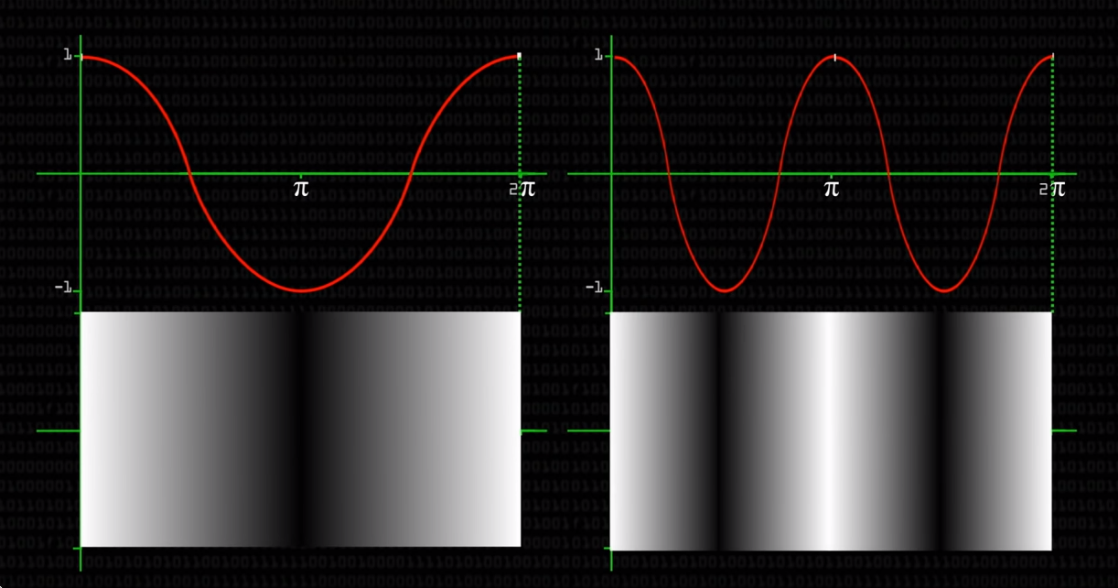
\includegraphics[width=\textwidth]{figs/freq_1.png}
        \caption{توصیف فرکانسی توابع 
        $\cos (x) , \cos (2x)$ \cite{youtube}}
        \label{freq_1}
\end{figure}

\begin{figure}[]
        \centering
        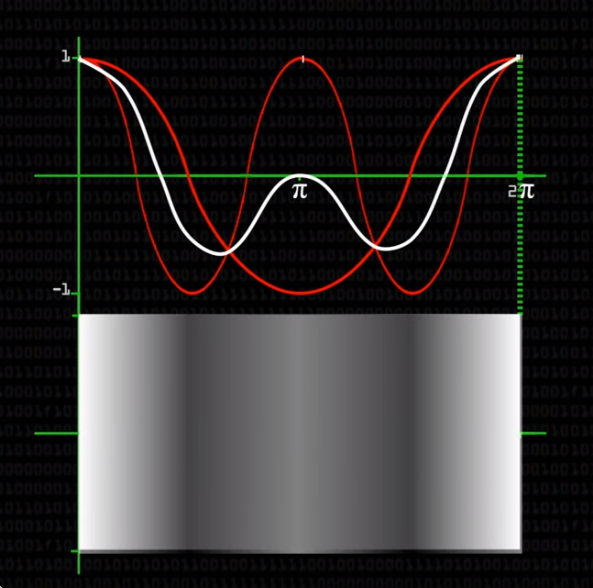
\includegraphics[width=0.5\textwidth]{figs/freq_2.png}
        \caption{توصیف فرکانسی تابع 
        $\cos (x) + \cos (2x) / 2$ \cite{youtube}}
        \label{freq_2}
\end{figure}

\section{نحوهٔ کار JPEG}
برای فشرده‌سازی یک تصویر در JPEG 
مراحل زیر انجام می‌شود. 

\begin{itemize}
        \item تبدیل تصویر به بلوک‌های کوچک 
        \item تبدیل هر بلوک به مجموعه‌ای از توابع کسینوسی استاندارد با DCT
        \item تنظیم ضرایب متناسب برای بلوک‌های DCT 
        \item کمپرس کردن ضرایب با استفاده از Huffman
\end{itemize}

\section{یک مثال از فشرده‌سازی JPEG}
برای درک بهتر مراحل گفته شده تلاش می‌کنیم تا ماتریس زیر را - که تصویر کانال خاکستری آن را در شکل 
\ref{jpeg_example}
مشاهده می‌شود -
را با الگوریتم‌های گفته‌شده فشرده‌سازی کنیم.
\begin{figure}[]
        \centering
        
\includegraphics[width=0.5\textwidth]{figs/jpeg_block.png}
        \caption{نمونهٔ تصویر برای فشرده‌سازی \cite{jpeg_example}}
        \label{jpeg_example}
\end{figure}
\[
        M = \begin{bmatrix}
                52 & 55 & 61 & 66 & 70 & 61 & 64 & 73\\
                63 & 59 & 55 & 90 & 109 & 85 & 69 & 72 \\
                62 & 59 & 68 & 113 & 144 & 104 & 66 & 73 \\
                63 & 58 & 71 & 122 & 154 & 106 & 70 & 60 \\
                67 & 61 & 68 & 104 & 126 & 88 & 68 & 70 \\
                79 & 65 & 60 & 70 & 77 & 68 & 58 & 75 \\
                85 & 71 & 64 & 59 & 55 & 61 & 65 & 83 \\
                87 & 79 & 69 & 68 & 65 & 76 & 78 & 94 

        \end{bmatrix}
\]
هر عنصر این ماتریس عددی بین ۰ تا ۲۵۵ دارد اما از آنجایی که تابع کسینوسی 
مقادیر بین ۱- تا ۱ می‌گیرد نیازمندیم تا با کم کردن هر عنصر این ماتریس از 
۱۲۸ 
هر عنصر این ماتریس را به عددی بین ۱۲۷- تا ۱۲۸ تبدیل کنیم.
ماتریس تبدیل‌شده به شکل زیر است.

\[
        M_{shifted} = \begin{bmatrix}
                -76 & -73 & -67 & -62 & -58 & -67 & -64 & -55\\
                -65 & -69 & -73 & -38 & -19 & -43 & -59 & -56 \\
                -66 & -69 & -60 & -15 & 16 & -24 & -62 & -55 \\
                -65 & -70 & -57 & -6 & 26 & -22 & -58 & -59 \\
                -61 & -67 & -60 & -24 & -2 & -40 & -60 & -58 \\
                -49 & -63 & -68 & -58 & -51 & -60 & -70 & -53 \\
                -43 & -57 & -64 & -69 & -73 & -67 & -63 & -45 \\
                -41 & -49 & -59 & -60 & -63 & -52 & -50 & -34 

        \end{bmatrix}
\]

در گام بعدی مقادیر این ماتریس را با استفاده از الگوریتم 
DCT به فضای فرکانس می‌بریم
هر مقدار از این ماتریس جدید برابر با ضریب فرکانس معادل در ماتریس 
استاندارد است. 

\[
        F = \begin{bmatrix}
                -415.38 & -30.19 & -61.20 & 27.24 & 56.12 & -20.10 & -2.39 & 0.46\\
                4.47 & -21.28 & -60.76 & 10.25 & 13.15 & -7.09 & -8.54 & 4.88 \\
                -46.83 & 7.37 & 77.13 & -24.56 & -28.91 & 9.93 & 5.42 & -5.65 \\
                -48.53 & 12.07 & 34.10 & -14.76 & -10.24 & 6.30 & 1.83 & 1.95 \\
                12.12 & -6.55 & -13.20 & -3.95 & -1.87 & 1.75 & -2.79 & 3.14 \\
                -7.73 & 2.91 & 2.38 & -5.94 & -2.38 & 0.94 & 4.30 & 1.85 \\
                -1.03 & 0.18 & 0.42 & -2.42 & -0.88 & -3.02 & 4.12 & -0.66 \\
                -0.17 & 0.14 & -1.07 & -4.19 & -1.17 & -0.10 & 0.50 & 1.68 

        \end{bmatrix}
\]
هر کدام از عناصر ماتریس بالا مقدار ضریب تاثیر فرکانس نشان‌داده‌شده در شکل 
\ref{freq_3} 
می‌باشند. 

\begin{figure}[]
        \centering
        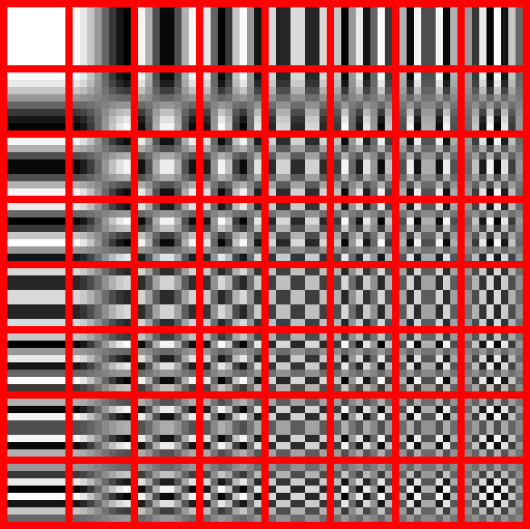
\includegraphics[]{figs/freq_3.png}
        \caption{ماتریس فرکانس‌های استاندارد \cite{standard_freqs}}
        \label{freq_3}
\end{figure}

تا به این لحظه هیچ مقداری از داده را برای فشره‌سازی از دست نداده‌ایم اما 
در این گام می‌خواهیم قسمت‌هایی از تصویر که برای چشم انسان قابل تشخیص نیستند
را حذف کنیم تا مقدار دادهٔ کمتری را ذخیره کنیم. 
باید توجه داشت که چشم انسان معمولا قادر به تشخصی و تمیز تصاویر با فرکانس‌های بالا در 
تصاویر نیست و همان‌طور که در ماتریس هم مشاهده می‌شود ضریب این فرکانس‌ها نسبت 
به فرکانس‌های پایین بسیار کم است، می‌توانید به مقدار بسیار بزرگ ۴۱۵ برای
فرکانس بسیار پایین در راستای x و y در ماتریس توجه کنید تا 
این نکته روشن شود. حال باید ضرایب فعلی ماتریس را با تقریبی گرد کنیم و تاثیر 
فرکانس‌های بالا را کمتر از تاثیر فرکانس‌های پایین قرار دهیم، از این رو 
از جدولی به نام
\lr{Quantization Table}
استفاده می‌کنیم. 

\subsection{\lr{Quantization Table}}
\lr{Quantization table}
جدولی است که در آن مقدار تاثیر هر فرکانس برای هر ردهٔ فشرده‌سازی 
برای عکس‌های JPEG به صورت جهانی استانداردسازی و تعیین شده‌است. 
برای مثال برای نرخ کمپرس ۵۰ درصد 
\lr{Quantization Table} 
به شکل زیر است. 

\[
        Q = \begin{bmatrix}
                16 & 11 & 10 & 16 & 24 & 40 & 51 & 61\\
                12 & 12 & 14 & 19 & 26 & 58 & 60 & 55 \\
                14 & 13 & 16 & 24 & 40 & 57 & 69 & 56 \\
                14 & 17 & 22 & 29 & 51 & 87 & 80 & 62 \\
                18 & 22 & 37 & 56 & 68 & 109 & 103 & 77 \\
                24 & 35 & 55 & 64 & 81 & 104 & 113 & 92 \\
                49 & 64 & 78 & 87 & 103 & 121 & 120 & 101 \\
                72 & 92 & 95 & 98 & 112 & 100 & 103 & 99 

        \end{bmatrix}
\]

حال برای آخرین گام باید مقادیر ماتریس
Q 
را بر مقادیر ماتریس F 
تقسیم کنیم و عدد به دست آمده را گرد کنیم. ماتریس نهایی برای فشرده‌سازی به شکل زیر است.

\[
       R = \begin{bmatrix}
                -26 & -3 & -6 & 2 & 2 & -1 & 0 & 0\\
                0 & -2 & -4 & 1 & 1 & 0 & 0 & 0 \\
                -3 & 1 & 5 & -1 & -1 & 0 & 0 & 0 \\
                -3 & 1 & 2 & -1 & 0 & 0 & 0 & 0 \\
                1 & 0 & 0 & 0 & 0 & 0 & 0 & 0 \\
                0 & 0 & 0 & 0 & 0 & 0 & 0 & 0 \\
                0 & 0 & 0 & 0 & 0 & 0 & 0 & 0 \\
                0 & 0 & 0 & 0 & 0 & 0 & 0 & 0 \\

        \end{bmatrix}
\]

همان‌طور که در ماتریس R مشهود است تعداد بسیار زیادی از عناصر ماتریس جدید
مقدار صفر دارند (که بیشتر فرکانس‌های بالا را شامل می‌شوند)
در ادامهٔ فشرده‌سازی این ماتریس به وسیلهٔ الگوریتم فشرده‌‌سازی بدون هدررفت داده
Huffman 
فشرده می‌شود و به همراه مقداری 
دادهٔ افزوده 
\footnote{\lr{meta data}}
مانند درصد فشرده‌سازی و... ذخیره می‌شود. 

\section{فشرده‌سازی Huffman}
برای این که ماتریس مرحلهٔ آخر را به یک رشتهٔ متنی تبدیل کنیم می‌خواهیم از 
فشرده‌سازی یا الگوریتم Huffman استفاده کنیم.
در این قسمت مختصرا الگوریتم Huffman برای فشرده‌سازی یک رشتهٔ متنی شرح داده می‌شود.

\subsection{تعریف}
برای نمایش رشته در حالت 
ascii 
برای هر حرف ۸ بیت فضا گرفته می‌شود و تمامی حروف با یک آرایهٔ هشت‌بیتی
نمایش داده می‌شوند. رشتهٔ زیر را در نظر بگیرید.
\begin{center}
        $S = bananasc$
\end{center}

در این رشته در حالت ascii به 
$ 8 * 8 = 64$ 
بیت فضا نیاز داریم، در صورتی که بخواهیم از طراحی 
با طول بیت ثابت برای هر حرف در این رشته استفاده کنیم می‌توانیم نظیرسازی 
زیر را در نظر بگیریم. 

\begin{table}[h]
        \centering
        \caption{نوعی نظیرسازی حروف با طول ثابت برای هر حرف}
        \label{huffman}
        \begin{tabular}{ll}
        \hline
        نماد & حرف \\ \hline
        001 & a \\
        010 & b \\
        011 & n \\
        100 & s \\
        101 & c \\ \hline
        \end{tabular}
\end{table}

در این روش برای نشان دادن هر حرف به سه بیت فضا نیاز داریم و در کل به
$ 8 * 3 = 24 $
بیت فضا نیاز داریم. 

اما در صورتی که به صورت دقیق‌تر به رشته نگاه کنیم متوجه می‌شویم که تعداد تکرار هر حرف
یکسان نیست و می‌توانیم برای نشان دادن هر حرف از تعداد بیت متغیر استفاده کنیم به شکلی که 
حروفی که بیشتر تکرار شده‌اند تعداد بیت کمتری بگیرند و حروفی که کمتر تکرار
شده اند از تعداد بیت بیشتری برای ذخیره‌‌سازی استفاده کنند. مثلا نظیرسازی زیر 
را برای این رشته در نظر بگیرید.

\begin{table}[h]
        \centering
        \caption{نوعی نظیرسازی حروف با طول متغیر برای هر حرف}
        \label{huffman}
        \begin{tabular}{ll}
        \hline
        نماد & حرف \\ \hline
        0 & a \\
        110 & b \\
        10 & n \\
        111 & s \\
        1110 & c \\ \hline
        \end{tabular}
\end{table}

درصورتی که رشتهٔ اصلی را با این نظیرسازی فشرده کنیم به بیت‌های زیر می‌رسیم.

\begin{center}
        $110010001001111110$
\end{center}

همان‌طور که در رشتهٔ جدید مشهود است تعداد بیت‌های استفاده‌شده برای نمایش
رشتهٔ اصلی به ۱۸ بیت کاهش پیدا کرده، نکته اساسی در این فشرده‌سازی 
این است که رشته به صورت یکتا قابل بازیابی باشد، در صورتی که به رشتهٔ بالا
دقت کنیم متوجه می‌شویم که تنها حالتی که می‌توان با توجه به حروف جدول برای
بازیابی بیت‌ها متصور شد همین حالتی‌ست که به رشتهٔ اصلی منجر می‌شود، این اتفاق به این دلیل
رخ می‌دهد که شروع هیچ حرفی زیرمجموعهٔ پیشوندی هیچ رشتهٔ دیگری نیست، 
برای مثال در صورتی که حرف a با 
$0$ 
و حرف b
با 
$010$ 
و حرف 
n 
با 
$10$ 
نمایش داده می‌شدندبرای رشتهٔ بیتی 
$010$
دو حالت
$an$
و 
$b$
می‌توانستیم متصور شویم، علت این اتفاق این است که رشتهٔ حرف 
a 
زیرمجموعهٔ حرف 
b
است. 

کلیت الگوریتم Huffman پیدا کردن بهترین کدگذاری برای هر حرف در رشتهٔ اصلی 
است که طول رشتهٔ نهایی کم‌ترین اندازه را داشته باشد، برای این کار از شبه کد زیر استفاده می‌شود.
\cite{huffman}
\vspace{5mm}

\begin{code}
//Huffman Algorithm
n := |C|;
Q := C;
for i := 1 to n − 1 do
        allocate a new node z
        z.lef t := x := Extract-Min(Q);
        z.right := y := Extract-Min(Q);
        z.freq := x.freq + y.freq;
        Insert(Q, z);
end for
return Extract-Min(Q); {return the root of the tree}
\end{code}
\vspace{5mm}
شکل 
\ref{huffman_tree}
مراحل الگوریتم Huffman را نشان می‌دهد.

\begin{figure}[]
        \centering
        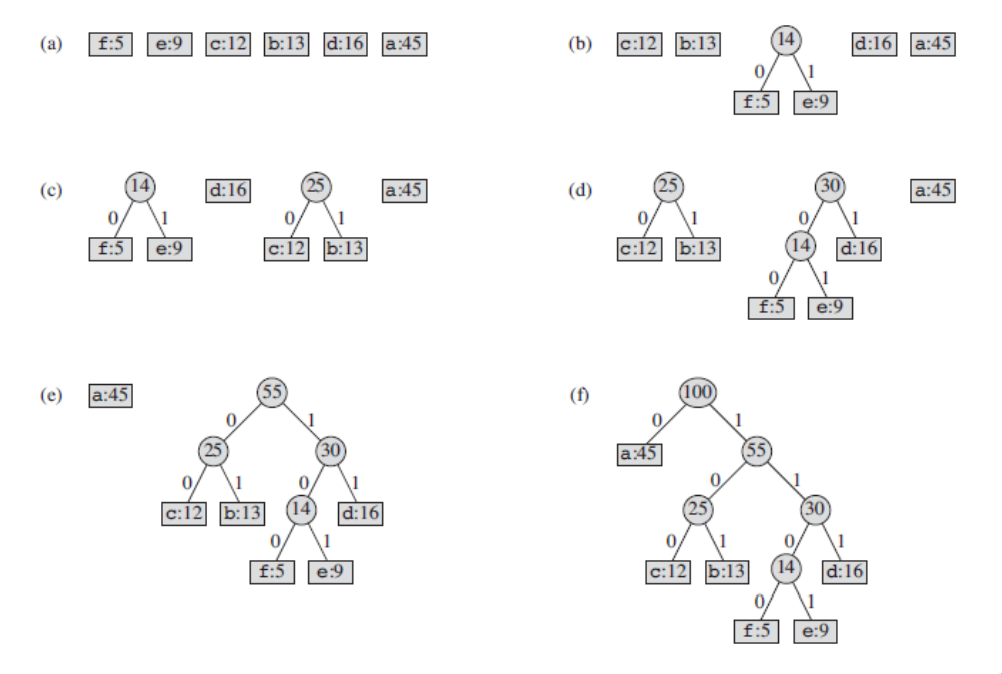
\includegraphics[width=\textwidth]{figs/huffamn_tree.png}
        \caption{مراحل الگوریتم Huffman \cite{huffman_tree}}
        \label{huffman_tree}
\end{figure}

